% !TeX program = LuaLaTeX
\documentclass[oneside]{book}
\usepackage{comment} % enables the use of multi-line comments (\ifx \fi) 
\usepackage{lipsum} %This package just generates Lorem Ipsum filler text. 
\usepackage[left=0.5in,right=2.5in,marginparwidth=2in]{geometry}
\usepackage{amsmath}
\usepackage{amssymb,amsthm}  % assumes amsmath package installed
\newtheorem{theorem}{Theorem}
\newtheorem{corollary}{Corollary}
\usepackage{graphicx}
\usepackage{tikz}
\usetikzlibrary{arrows}
\usepackage{verbatim}
\usepackage{float}
\usepackage{tikz}
    \usetikzlibrary{shapes,arrows}
    \usetikzlibrary{arrows,calc,positioning}

    \tikzset{
        block/.style = {draw, rectangle,
            minimum height=1cm,
            minimum width=1.5cm},
        input/.style = {coordinate,node distance=1cm},
        output/.style = {coordinate,node distance=4cm},
        arrow/.style={draw, -latex,node distance=2cm},
        pinstyle/.style = {pin edge={latex-, black,node distance=2cm}},
        sum/.style = {draw, circle, node distance=1cm},
    }
\usepackage{xcolor}
\usepackage{mdframed}
\usepackage[shortlabels]{enumitem}
\usepackage{indentfirst}
\usepackage{hyperref}
\usepackage{mhchem}
\usepackage{titlesec}
\usepackage{fontspec}
\usepackage{titlesec, blindtext, color}
\usepackage{tcolorbox}
\usepackage{caption}
\usepackage{sidenotes} 
\usepackage{esdiff}
\renewcommand{\thesubsection}{\thesection.\alph{subsection}}
\usepackage{esvect}
\usepackage{pdfpages}

\usepackage{physics}
\usepackage{amsmath}
\usepackage{tikz}
\usepackage{mathdots}
\usepackage{yhmath}
\usepackage{cancel}
\usepackage{color}
\usepackage{siunitx}
\usepackage{array}
\usepackage{multirow}
\usepackage{amssymb}
\usepackage{gensymb}
\usepackage{tabularx}
\usepackage{extarrows}
\usepackage{booktabs}
\usetikzlibrary{fadings}
\usetikzlibrary{patterns}
\usetikzlibrary{shadows.blur}
\usetikzlibrary{shapes}

\renewcommand{\qed}{\quad\qedsymbol}
\setlength\parindent{0pt}


\begin{document}
\begin{titlepage}
    \includepdf[fitpaper]{graphics/cover}
\end{titlepage}
\clearpage

%\setmainfont{KITTY CAT}
%\setmainfont{Cedarville Cursive}
\setmainfont{Indie Flower}

\tableofcontents

\chapter{Introduction}
\section{Why statistical inference?}
There are three main questions we would like to answer:
\begin{enumerate}
    \item Given a random vector $X$, determine which $\theta\in \Theta$ is most compatible with the data given [i.e. which $\theta\in\Theta$ generates $X$]. This is point estimation.
    \item Given an $X$ we wish to determine if a given value of $\theta$ or distribution $f_\theta$ is consistent. This is hypothesis testing.
    \item After (1), we would like to find a suitable rang of values of $\theta$ which is compatible. This is interval estimation.
\end{enumerate}
We would also like our answers to be optimal in each of the above cases. 

\section{Problem of non-indetifiability}
This is a problem which arises when more than one value of $\theta\in\Theta$ can give rise to the same $f_\theta$. 

\begin{center}
    \tikzset{every picture/.style={line width=0.75pt}} %set default line width to 0.75pt        

    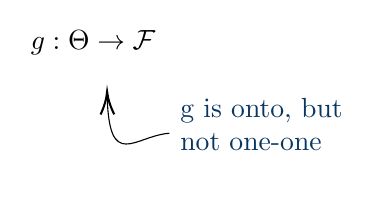
\begin{tikzpicture}[x=0.75pt,y=0.75pt,yscale=-1,xscale=1]
    %uncomment if require: \path (0,300); %set diagram left start at 0, and has height of 300
    
    %Curve Lines [id:da8212179968196289] 
    \draw    (190,190) .. controls (173.26,191.23) and (160.88,208.71) .. (160.03,171.73) ;
    \draw [shift={(160,170)}, rotate = 89.27] [color={rgb, 255:red, 0; green, 0; blue, 0 }  ][line width=0.75]    (10.93,-3.29) .. controls (6.95,-1.4) and (3.31,-0.3) .. (0,0) .. controls (3.31,0.3) and (6.95,1.4) .. (10.93,3.29)   ;
    
    % Text Node
    \draw (122,139.4) node [anchor=north west][inner sep=0.75pt]    {$g:\Theta \rightarrow \mathcal{F}$};
    % Text Node
    \draw (194,172) node [anchor=north west][inner sep=0.75pt]   [align=left] {\textcolor[rgb]{0.03,0.21,0.38}{g is onto, but}\\\textcolor[rgb]{0.03,0.21,0.38}{ not one-one}};
    
    
    \end{tikzpicture}
    
\end{center}


$\exists \theta_1,\theta_2$ such that $g(\theta_1)=g(\theta_2)$. The difficulty arising from this is very obvious: with non-identifiability, $\theta_1$ can be confused with $\theta_2$ as we are essentially claiming that both $\theta_1$ and $\theta_2$ results in the same data generating mechanism.  \textbf{We must understand that this is an inherent problem of our data generating mechanism/experiment and must be addressed before any further analysis is carried out.} 

\subsection{Example}
Consider a scenario where we want to test the effectiveness of two fertilizers on a field. What we might do is divide the field in two divisions such, use fertilizer one on the first half and fertilizer two on the second half and then record our crop yield. Assume that the field has yield follows a normal distribution with mean $\alpha$ with standard deviation $1$. Further, assume that each fertilizer $i$ increases yield by $\alpha_i$. We repeat this process several($=n$) times.


\begin{marginfigure}%
        

    % Pattern Info
     
    \tikzset{
        pattern size/.store in=\mcSize, 
        pattern size = 5pt,
        pattern thickness/.store in=\mcThickness, 
        pattern thickness = 0.3pt,
        pattern radius/.store in=\mcRadius, 
        pattern radius = 1pt}
        \makeatletter
        \pgfutil@ifundefined{pgf@pattern@name@_sfjfqfpww}{
        \pgfdeclarepatternformonly[\mcThickness,\mcSize]{_sfjfqfpww}
        {\pgfqpoint{0pt}{0pt}}
        {\pgfpoint{\mcSize+\mcThickness}{\mcSize+\mcThickness}}
        {\pgfpoint{\mcSize}{\mcSize}}
        {
        \pgfsetcolor{\tikz@pattern@color}
        \pgfsetlinewidth{\mcThickness}
        \pgfpathmoveto{\pgfqpoint{0pt}{0pt}}
        \pgfpathlineto{\pgfpoint{\mcSize+\mcThickness}{\mcSize+\mcThickness}}
        \pgfusepath{stroke}
        }}
        \makeatother
        
        % Pattern Info
         
        \tikzset{
        pattern size/.store in=\mcSize, 
        pattern size = 5pt,
        pattern thickness/.store in=\mcThickness, 
        pattern thickness = 0.3pt,
        pattern radius/.store in=\mcRadius, 
        pattern radius = 1pt}
        \makeatletter
        \pgfutil@ifundefined{pgf@pattern@name@_mho7itfp5}{
        \pgfdeclarepatternformonly[\mcThickness,\mcSize]{_mho7itfp5}
        {\pgfqpoint{0pt}{0pt}}
        {\pgfpoint{\mcSize+\mcThickness}{\mcSize+\mcThickness}}
        {\pgfpoint{\mcSize}{\mcSize}}
        {
        \pgfsetcolor{\tikz@pattern@color}
        \pgfsetlinewidth{\mcThickness}
        \pgfpathmoveto{\pgfqpoint{0pt}{0pt}}
        \pgfpathlineto{\pgfpoint{\mcSize+\mcThickness}{\mcSize+\mcThickness}}
        \pgfusepath{stroke}
        }}
        \makeatother
        \tikzset{every picture/.style={line width=0.75pt}} %set default line width to 0.75pt        
        
        \begin{tikzpicture}[x=0.75pt,y=0.75pt,yscale=-1,xscale=1]
        %uncomment if require: \path (0,300); %set diagram left start at 0, and has height of 300
        
        %Shape: Rectangle [id:dp9553632390766091] 
        \draw   (190,60) -- (310,60) -- (310,180) -- (190,180) -- cycle ;
        %Shape: Rectangle [id:dp6238306915981553] 
        \draw  [pattern=_sfjfqfpww,pattern size=6pt,pattern thickness=0.75pt,pattern radius=0pt, pattern color={rgb, 255:red, 61; green, 106; blue, 12}] (190,60) -- (250,60) -- (250,180) -- (190,180) -- cycle ;
        %Shape: Rectangle [id:dp7361739770556295] 
        \draw  [color={rgb, 255:red, 9; green, 46; blue, 132 }  ,draw opacity=1 ][pattern=_mho7itfp5,pattern size=6pt,pattern thickness=0.75pt,pattern radius=0pt, pattern color={rgb, 255:red, 74; green, 144; blue, 226}] (250,60) -- (310,60) -- (310,180) -- (250,180) -- cycle ;
        %Curve Lines [id:da3829501751065828] 
        \draw    (321.19,108.23) .. controls (359.69,50.34) and (319.7,30.25) .. (290,30) ;
        \draw [shift={(320,110)}, rotate = 304.35] [color={rgb, 255:red, 0; green, 0; blue, 0 }  ][line width=0.75]    (10.93,-3.29) .. controls (6.95,-1.4) and (3.31,-0.3) .. (0,0) .. controls (3.31,0.3) and (6.95,1.4) .. (10.93,3.29)   ;
        %Curve Lines [id:da2851128639217373] 
        \draw    (190,210) .. controls (165.74,182.03) and (140.51,160.44) .. (178.82,130.9) ;
        \draw [shift={(180,130)}, rotate = 143.13] [color={rgb, 255:red, 0; green, 0; blue, 0 }  ][line width=0.75]    (10.93,-3.29) .. controls (6.95,-1.4) and (3.31,-0.3) .. (0,0) .. controls (3.31,0.3) and (6.95,1.4) .. (10.93,3.29)   ;
        
        % Text Node
        \draw (189,22) node [anchor=north west][inner sep=0.75pt]   [align=left] {Use Fertilizer 2};
        % Text Node
        \draw (199,201) node [anchor=north west][inner sep=0.75pt]   [align=left] {Use Fertilizer 1};
        
        
        \end{tikzpicture}
\end{marginfigure}%

Assume on the $j^{th}$ iteration with fertilizer $i$ the yield is $X_{ij}$. Define $X_1=[X_{11},X_{12},X_{13}\hdots X_{1n}]$ and $X_2=[X_{21},X_{22},X_{23}\hdots X_{2n}]$. Then by using our setup, we can use $X_1$ and $X_2$ to estimate $\alpha+\alpha_1$ and $\alpha+\alpha_2$ but not $\alpha,\alpha_1,\alpha_2$ individually.
\begin{center}
    

\tikzset{every picture/.style={line width=0.75pt}} %set default line width to 0.75pt        

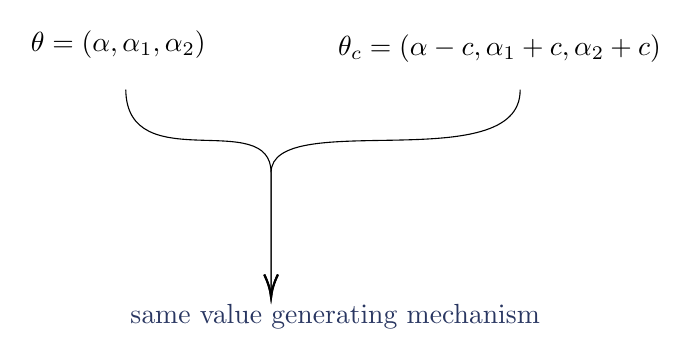
\begin{tikzpicture}[x=0.75pt,y=0.75pt,yscale=-1,xscale=1]
%uncomment if require: \path (0,300); %set diagram left start at 0, and has height of 300

%Curve Lines [id:da9164633896150238] 
\draw    (160,100) .. controls (160.5,143.25) and (230,108.25) .. (230,140) .. controls (230,170.96) and (230,172.68) .. (230,198) ;
\draw [shift={(230,200)}, rotate = 270] [color={rgb, 255:red, 0; green, 0; blue, 0 }  ][line width=0.75]    (10.93,-3.29) .. controls (6.95,-1.4) and (3.31,-0.3) .. (0,0) .. controls (3.31,0.3) and (6.95,1.4) .. (10.93,3.29)   ;
%Curve Lines [id:da6639974611294849] 
\draw    (350,100) .. controls (350.5,143.25) and (230,108.25) .. (230,140) .. controls (230,170.96) and (230,172.68) .. (230,198) ;
\draw [shift={(230,200)}, rotate = 270] [color={rgb, 255:red, 0; green, 0; blue, 0 }  ][line width=0.75]    (10.93,-3.29) .. controls (6.95,-1.4) and (3.31,-0.3) .. (0,0) .. controls (3.31,0.3) and (6.95,1.4) .. (10.93,3.29)   ;

% Text Node
\draw (113,70.4) node [anchor=north west][inner sep=0.75pt]    {$\theta =( \alpha ,\alpha _{1} ,\alpha _{2})$};
% Text Node
\draw (261,72.4) node [anchor=north west][inner sep=0.75pt]    {$\theta _{c} =( \alpha -c,\alpha _{1} +c,\alpha _{2} +c)$};
% Text Node
\draw (161,202) node [anchor=north west][inner sep=0.75pt]  [color={rgb, 255:red, 40; green, 54; blue, 97 }  ,opacity=1 ] [align=left] {\textcolor[rgb]{0.16,0.21,0.38}{same value generating mechanism}};


\end{tikzpicture}

\end{center}
Again note this inability is an inherent flaw in the experiment itself, and we can't do anything to circumnavigate it.  However, we might address this problem by assuming that $\alpha_1+\alpha_2=0$. Note, this is definitely not true. But we are claiming something along the lines that the net fertility remains constant, and this helps in computing all the values. 



\section{Parameter}
A parameter is a function $$\nu:\mathcal{F}_\theta\to\mathcal N$$
where $\mathcal N$ is an arbitrary set. When $F_\theta$ is an identifiable parameterization, then there exists function $q$ such that:
$$\nu(F_\theta)=q(\theta)$$
\subsection{Examples}
\begin{enumerate}
    \item $\mu(\theta)=\int xdF_\theta(x)$
    \item $\sigma^2(\theta)=\int x^2dF_\theta(x)-(\mu(\theta)^2)$
    \item $m(\theta)=$ median of $F_\theta$
\end{enumerate}

\section{Regular families}
For our work we will assume that:
\begin{enumerate}
    \item All $F_\theta\in\mathcal F$ have continuous CDF with density $f_\theta$ or are discrete with pmf $f_\theta$
    \item There is identifiable parameterization. 
\end{enumerate}


\chapter{Statistic}
\section{Introduction}
Any measurable function $T:X\to \mathbb R^k$ is called a statistic. 

The idea is to compress the given data without losing valuable information. We look at two extreme cases:
\begin{itemize}
    \item $T(X)=$constant: This tells us nothing and all information is lost,
    \item $T(X)=X$: while this retains all information, there is no compression that takes place. 
\end{itemize}

\section{Ancillary Statistics}
We wish to find good statistics. And it turns out that to achieve this it is better to sieve out the bad ones and then look further in whatever is left$^*$.\\
\begin{marginfigure}%
    \footnotesize $^*$Honestly, this feels like something you find on cleanup: You do everything and then understand that doing it this way is smoother.
\end{marginfigure}%


An ancillary statistic $T=T(X)$ is such that the distribution of $T(X)$ is independent of $\theta$. 
\subsection{Example 1}
Assume $X_1,X_2\hdots X_n\sim\mathcal(\mu,1),\mu\in\mathbb R$. Let
$$T(X)=\sum_{i=0}^n\sum_{j=0}^n(X_i-X_j)^2$$ 
Two approaches for solving this are:
\begin{enumerate}
    \item Define $\tilde{X_i}=X_i-\bar X$. Note that:
        \begin{align*}
            T(X)&=\sum_{i\ne j}(X_i-X_j)\\
            &=\sum_{i\ne j}(\tilde{X_i}-\tilde{X_j})\\
            &=(n-1)\sum_{i}\tilde{X_i}^2-2\sum_{i\ne j}\tilde{X_i}\tilde{X_j}\\
            &=(n+1)\sum_{i}\tilde{X_i}^2-2\sum_{i,j}\tilde{X_i}\tilde{X_j}\\
            &=(n+1)\sum_{i}\tilde{X_i}^2-2\left(\sum_{i}\tilde{X_i}\right)\left(\sum_{j}\tilde{X_j}\right)\\
            &=(n+1)\sum_{i}\left(X_i-\bar X\right)
        \end{align*}
        Now distribution of $X_i-\bar X\sim\mathcal N(0,1)$ which is independent of $\mu$. Therefore, $T$ is ancillary.
    \item The above argument can be considerable shortened by arguing that the distribution of $X_i-X_j$ is independent of $\mu$, and therefore the whole sum is independent of $\mu$.
\end{enumerate}
\subsection{Example 2}
Assume $X_1,X_2\hdots X_n\sim Exp(\theta)$. The density function is given by: $f_\theta(x)=\theta e^{-\theta x}$. Such a distribution often occurs when modelling things like lifetime of a particular make of a bulb, etc. Define:
$$T(X)=\frac{\max_i X_i}{\min_i X_i}$$
Finding the distribution of $T$ explicitly is a nightmare. Instead, what we do is define $Y_i=\theta X_i$. Note that:
\begin{align*}
    P(Y_i<y)=P(\theta X_i<y)=\int_0^{y/\theta}\theta e^{-\theta x}dx=\int_0^ye^{-u}du
\end{align*}
Therefore, $Y_i\sim Exp(1)$. We rewrite $T$ as:

$$T(X)=\frac{\max_i X_i}{\min_i X_i}=\frac{\max_i Y_i}{\min_i Y_i}=T(Y)$$
But, it is trivial to note that any parameter on $Y$ is independent of $\theta$. Therefore, $T(X)$ is ancillary. 

\subsection{Example 3}
Assume $X_1,X_2\hdots X_n\sim Unif(0,\theta)$. Define:
$$T(X)=\frac{\max_i X_i}{\min_i X_i}$$
Define $Y_i=X_i/\theta$. Note that:
\begin{align*}
    P(Y_i<y)=P(X_i/\theta <y)=\int_0^{y\theta}\frac{1}{\theta}dx=\int_0^y du
\end{align*}
Therefore, $y\sim Unif(0,1)$. We rewrite $T$ as:

$$T(X)=\frac{\max_i X_i}{\min_i X_i}=\frac{\max_i Y_i}{\min_i Y_i}=T(Y)$$
Again as any parameter on $Y$ is independent of $\theta$. Therefore, $T(X)$ is ancillary. 

The idea in the examples above is that we are "scaling" the function to fit our needs. 
\section{Scale Family}
A scale family is a family $\mathcal F$ of distribution given by:
$$\left\{f_\theta|f_\theta(x)=\frac{1}{\theta}g\left(\frac{x}{\theta}\right)\right\}$$
Where $g$ is a known distribution. Set $Y_i=X_i/\theta$. Any $T(X)$ which can be written as $S(Y)$ is ancillary. 

\section{Location Family}
A scale family is a family $\mathcal F$ of distribution given by:
$$\left\{f_\theta|f_\theta(x)=g\left(x-\theta\right)\right\}$$
Where $g$ is a known distribution. Set $Y=X_i-\theta$. Any $T(X)$ which can be written as $S(y)$ is ancillary. 


\section{Location-Scale Family}
A scale family is a family $\mathcal F$ of distribution given by:
$$\left\{f_\theta|f_\theta(x)=\frac{1}{\sigma}g\left(\frac{x-\mu}{\sigma}\right)\right\}$$
Where $g$ is a known distribution. Set $Y_i=(X_i-\mu)/\sigma$. Any $T(X)$ which can be written as $S(Y)$ is ancillary. 

\section{Limiting conditions}
Other ways of identifying a "bad-statisttic" is to look at limiting conditions. For example, let $X_i\sim Unif(0,\theta)$. Consider two candidates:
$$T_1(X)=\max_i X_i$$
$$T_2(X)=\min_i X_i$$
It is easy to compute that:
$$f_{T_2}(t)=\frac{n}{\theta}\left(1-\frac{t}{\theta}\right)^{n-1},0<t<\theta$$
$$f_{T_1}(t)=\frac{n}{\theta}\left(\frac{t}{\theta}\right)^{n-1},0<t<\theta$$
\begin{center}
    

\tikzset{every picture/.style={line width=0.75pt}} %set default line width to 0.75pt        

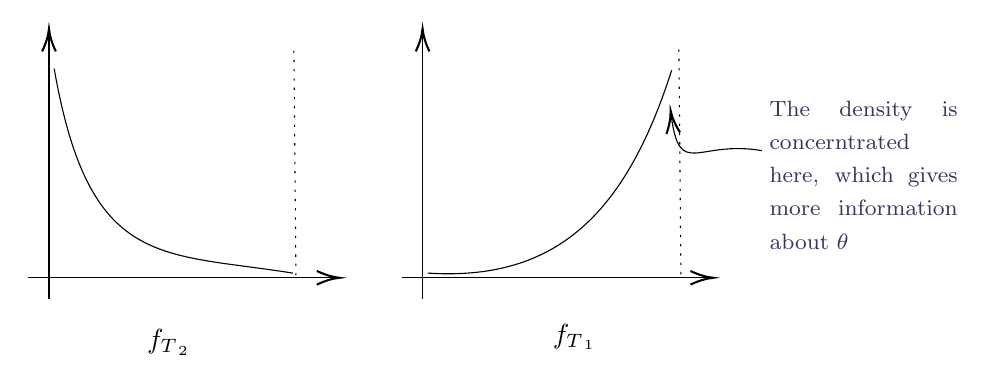
\begin{tikzpicture}[x=0.75pt,y=0.75pt,yscale=-1,xscale=1]
%uncomment if require: \path (0,300); %set diagram left start at 0, and has height of 300

%Straight Lines [id:da696613446369336] 
\draw    (50,180) -- (198,180) ;
\draw [shift={(200,180)}, rotate = 180] [color={rgb, 255:red, 0; green, 0; blue, 0 }  ][line width=0.75]    (10.93,-3.29) .. controls (6.95,-1.4) and (3.31,-0.3) .. (0,0) .. controls (3.31,0.3) and (6.95,1.4) .. (10.93,3.29)   ;
%Straight Lines [id:da1381343986177732] 
\draw    (60,190) -- (60,62) ;
\draw [shift={(60,60)}, rotate = 90] [color={rgb, 255:red, 0; green, 0; blue, 0 }  ][line width=0.75]    (10.93,-3.29) .. controls (6.95,-1.4) and (3.31,-0.3) .. (0,0) .. controls (3.31,0.3) and (6.95,1.4) .. (10.93,3.29)   ;
%Curve Lines [id:da4085954166909199] 
\draw    (62.5,79.25) .. controls (79.5,176) and (113.5,167.5) .. (177.5,177.75) ;
%Straight Lines [id:da25310792209645006] 
\draw    (230,180) -- (378,180) ;
\draw [shift={(380,180)}, rotate = 180] [color={rgb, 255:red, 0; green, 0; blue, 0 }  ][line width=0.75]    (10.93,-3.29) .. controls (6.95,-1.4) and (3.31,-0.3) .. (0,0) .. controls (3.31,0.3) and (6.95,1.4) .. (10.93,3.29)   ;
%Straight Lines [id:da8105666029275377] 
\draw    (240,190) -- (240,62) ;
\draw [shift={(240,60)}, rotate = 90] [color={rgb, 255:red, 0; green, 0; blue, 0 }  ][line width=0.75]    (10.93,-3.29) .. controls (6.95,-1.4) and (3.31,-0.3) .. (0,0) .. controls (3.31,0.3) and (6.95,1.4) .. (10.93,3.29)   ;
%Curve Lines [id:da6619730443236055] 
\draw    (242.5,177.75) .. controls (302,181.5) and (337,152.25) .. (360,80) ;
%Straight Lines [id:da8583418589836571] 
\draw  [dash pattern={on 0.84pt off 2.51pt}]  (363.5,70) -- (364.5,180.75) ;
%Straight Lines [id:da14841694409347916] 
\draw  [dash pattern={on 0.84pt off 2.51pt}]  (178,70.5) -- (179,181.25) ;
%Curve Lines [id:da983651205979652] 
\draw    (359.74,101.49) .. controls (363.83,132.94) and (372.14,113.36) .. (403.5,118.75) ;
\draw [shift={(359.5,99.5)}, rotate = 83.34] [color={rgb, 255:red, 0; green, 0; blue, 0 }  ][line width=0.75]    (10.93,-3.29) .. controls (6.95,-1.4) and (3.31,-0.3) .. (0,0) .. controls (3.31,0.3) and (6.95,1.4) .. (10.93,3.29)   ;

% Text Node
\draw (452.5,130.5) node   [align=left] {\begin{minipage}[lt]{68pt}\setlength\topsep{0pt}
{\footnotesize \textcolor[rgb]{0.22,0.21,0.38}{The density is concerntrated here, which gives more information about $\displaystyle \theta $}}
\end{minipage}};
% Text Node
\draw (106,203.4) node [anchor=north west][inner sep=0.75pt]    {$f_{T}{}_{_{2}}$};
% Text Node
\draw (301.5,200.9) node [anchor=north west][inner sep=0.75pt]    {$f_{T}{}_{_{1}}$};


\end{tikzpicture}

\end{center}


\section{Characterization in terms of level sets}
Consider a level set of $T$
$$A_t=\left\{x\in\mathbb R^n|T(x)=t \right\}$$

Ideally what we want is $T$ to do is compress all information about $\theta$ and leave out all the rest. This essentially translates to arguing that any variability of $x$ in $A$ is independent of $theta$, or more formally,  conditional distribution of $X$ given $T(X)=t$ is independent of $\theta$. But that implies that for any $t$, $T$ restricted to $T^{-1}(t)$ is ancillary in nature.

\begin{center}


% Pattern Info
 
\tikzset{
pattern size/.store in=\mcSize, 
pattern size = 5pt,
pattern thickness/.store in=\mcThickness, 
pattern thickness = 0.3pt,
pattern radius/.store in=\mcRadius, 
pattern radius = 1pt}
\makeatletter
\pgfutil@ifundefined{pgf@pattern@name@_ehq3pit3w}{
\pgfdeclarepatternformonly[\mcThickness,\mcSize]{_ehq3pit3w}
{\pgfqpoint{0pt}{0pt}}
{\pgfpoint{\mcSize+\mcThickness}{\mcSize+\mcThickness}}
{\pgfpoint{\mcSize}{\mcSize}}
{
\pgfsetcolor{\tikz@pattern@color}
\pgfsetlinewidth{\mcThickness}
\pgfpathmoveto{\pgfqpoint{0pt}{0pt}}
\pgfpathlineto{\pgfpoint{\mcSize+\mcThickness}{\mcSize+\mcThickness}}
\pgfusepath{stroke}
}}
\makeatother

% Pattern Info
 
\tikzset{
pattern size/.store in=\mcSize, 
pattern size = 5pt,
pattern thickness/.store in=\mcThickness, 
pattern thickness = 0.3pt,
pattern radius/.store in=\mcRadius, 
pattern radius = 1pt}
\makeatletter
\pgfutil@ifundefined{pgf@pattern@name@_c23r6jn40}{
\pgfdeclarepatternformonly[\mcThickness,\mcSize]{_c23r6jn40}
{\pgfqpoint{0pt}{0pt}}
{\pgfpoint{\mcSize+\mcThickness}{\mcSize+\mcThickness}}
{\pgfpoint{\mcSize}{\mcSize}}
{
\pgfsetcolor{\tikz@pattern@color}
\pgfsetlinewidth{\mcThickness}
\pgfpathmoveto{\pgfqpoint{0pt}{0pt}}
\pgfpathlineto{\pgfpoint{\mcSize+\mcThickness}{\mcSize+\mcThickness}}
\pgfusepath{stroke}
}}
\makeatother

% Pattern Info
 
\tikzset{
pattern size/.store in=\mcSize, 
pattern size = 5pt,
pattern thickness/.store in=\mcThickness, 
pattern thickness = 0.3pt,
pattern radius/.store in=\mcRadius, 
pattern radius = 1pt}
\makeatletter
\pgfutil@ifundefined{pgf@pattern@name@_cldnruwyf}{
\pgfdeclarepatternformonly[\mcThickness,\mcSize]{_cldnruwyf}
{\pgfqpoint{0pt}{0pt}}
{\pgfpoint{\mcSize+\mcThickness}{\mcSize+\mcThickness}}
{\pgfpoint{\mcSize}{\mcSize}}
{
\pgfsetcolor{\tikz@pattern@color}
\pgfsetlinewidth{\mcThickness}
\pgfpathmoveto{\pgfqpoint{0pt}{0pt}}
\pgfpathlineto{\pgfpoint{\mcSize+\mcThickness}{\mcSize+\mcThickness}}
\pgfusepath{stroke}
}}
\makeatother
\tikzset{every picture/.style={line width=0.75pt}} %set default line width to 0.75pt        

\begin{tikzpicture}[x=0.75pt,y=0.75pt,yscale=-1,xscale=1]
%uncomment if require: \path (0,300); %set diagram left start at 0, and has height of 300

%Shape: Rectangle [id:dp7650634010679893] 
\draw   (100,50) -- (320,50) -- (320,270) -- (100,270) -- cycle ;
%Shape: Polygon Curved [id:ds08761310440821968] 
\draw  [pattern=_ehq3pit3w,pattern size=6pt,pattern thickness=0.75pt,pattern radius=0pt, pattern color={rgb, 255:red, 50; green, 81; blue, 15}] (140,50) .. controls (152,50.13) and (205,50.75) .. (230,50) .. controls (255,49.25) and (172,124.25) .. (230,160) .. controls (288,195.75) and (293,269.75) .. (260,270) .. controls (227,270.25) and (163,269.75) .. (140,270) .. controls (117,270.25) and (228.5,228.25) .. (170,190) .. controls (111.5,151.75) and (128,49.88) .. (140,50) -- cycle ;
%Curve Lines [id:da3843341849099152] 
\draw    (360,120) .. controls (321.69,175.47) and (247.74,110.41) .. (200.71,169.11) ;
\draw [shift={(200,170)}, rotate = 307.96] [color={rgb, 255:red, 0; green, 0; blue, 0 }  ][line width=0.75]    (10.93,-3.29) .. controls (6.95,-1.4) and (3.31,-0.3) .. (0,0) .. controls (3.31,0.3) and (6.95,1.4) .. (10.93,3.29)   ;
%Shape: Polygon Curved [id:ds08995675669480385] 
\draw  [pattern=_c23r6jn40,pattern size=6pt,pattern thickness=0.75pt,pattern radius=0pt, pattern color={rgb, 255:red, 126; green, 211; blue, 33}] (320,50) .. controls (320,49.25) and (205,50.75) .. (230,50) .. controls (255,49.25) and (172,124.25) .. (230,160) .. controls (288,195.75) and (293,269.75) .. (260,270) .. controls (227,270.25) and (320,270.25) .. (320,270) .. controls (320,269.75) and (320,180.25) .. (320,180) .. controls (320,179.75) and (320,50.75) .. (320,50) -- cycle ;
%Shape: Polygon Curved [id:ds0748195172442584] 
\draw  [pattern=_cldnruwyf,pattern size=6pt,pattern thickness=0.75pt,pattern radius=0pt, pattern color={rgb, 255:red, 245; green, 166; blue, 35}] (140,50) .. controls (152,50.13) and (101,51.25) .. (100,50) .. controls (99,48.75) and (101,180.75) .. (100,180) .. controls (99,179.25) and (99.5,270.25) .. (100,270) .. controls (100.5,269.75) and (163.5,269.75) .. (140,270) .. controls (116.5,270.25) and (228.5,228.25) .. (170,190) .. controls (111.5,151.75) and (128,49.88) .. (140,50) -- cycle ;

% Text Node
\draw (362,77) node [anchor=north west][inner sep=0.75pt]   [align=left] {\textcolor[rgb]{0.21,0.22,0.38}{T is ancillary in a level set}\\\textcolor[rgb]{0.21,0.22,0.38}{(each shaded region). }\\\textcolor[rgb]{0.21,0.22,0.38}{Any vaiability }\\\textcolor[rgb]{0.21,0.22,0.38}{is independent of $\displaystyle \theta $ }};


\end{tikzpicture}

\end{center}
Such a $T$ is called a sufficient statistic.
\section{Sufficient Statistic}
$T=T(x)$ is said to be sufficient for $\theta$ if $P(X=B|T=t)$ is independent of $\theta$ for all $B\in\mathcal B_{\mathbb R^n},t\in\mathbb R^k$.
Note that any one-one map of a sufficient statistic is also sufficient.
\subsection{Example}
Let $X_1,X_2\hdots X_i$ be Bernoulli iid with parameter $\theta$, i.e.
$$P(X_i=1)=\theta\qquad P(X_i=0)=1-\theta$$
Take $T=\sum X_i$. We calculate $P(X=x_i|T=t)$. 
\begin{align*}
    P(X=x_i|T=t)=\frac{P(X=x,T(X)=t)}{P(T=t)}
\end{align*}
the denominator easily comes out to be ${n\choose t}\theta^t(1-\theta)^{n-t}$. For the numerator, consider two cases:
\begin{enumerate}
    \item $T(x)=t$: The event $[X=x]$ is a subset of $[T(x)=t]$. Therefore, the numerator simplifies to $P(X=x)=\theta^t(1-\theta)^{n-t}$, the whole expression simplifies to ${n\choose t}^{-1}$.
    \item $T(x)\ne t$: The events $[X=x]$ and $[T=t]$ are disjoint. Therefore, the numerator simplifies to 0.
\end{enumerate}
In either case, we see that the value of the expression is independent of $\theta$.

\section{Fisher-Neyman factorization}
Calculating conditional probabilities is hard for continuous distributions. Finding candidate $T$ for checking is even harder. A nice characterization for overcoming these difficulties is Fisher-Neyman factorization. $T(X)$ s sufficient for $X$ if and only if $f_\theta(x)$ can be written as 
$$f_\theta(x)=g(T(x),\theta)h(x)$$
\subsection{Example 1}
Let $X_i$s be iid Bernoulli with parameter $\theta$.

\begin{align*}
    f_\theta(x)&=P_\theta(X=x)\tag*{\text{[Good practice to include $\theta$ to show dependence]}}\\
    &=\prod_{i=1}^n\theta^{x_1}(1-\theta)^{1-x_i}1_{x_i\in\{0,1\}}\tag*{\text{[Make sure to characterize the domain]}}\\
    &=\underbrace{\theta^{\sum x_i}(1-\theta)^{n-\sum x_i}}_{\substack{\text{Set $T(x)=\sum x_i$} \\ \text{This part becomes $g(T(x),\theta)$}}}\underbrace{1_{x_i\in\{0,1\}}}_{\text{This becomes $h(x)$}}
\end{align*}
Which is exactly what we had concluded before. 
\subsection{Example 2}
Let $X_i$s be iid exponentials with parameter $\theta$.
$$f_\theta(x)=\prod \theta e^{-\theta x_i}1_{x_i>0}=\theta^ne^{-\theta\sum x_i}\prod 1_{x_i>0}$$
We have a similar decomposition as before with $T(x)=\sum x_i$
\subsection{Example 3}
Let $X_i$s be iid uniform with parameter $\theta$.
\begin{align*}
    f_\theta(x)=\prod_{i}\theta^{-1}1_{x_i\in(0,\theta)}\tag*{\text{[Note how the domain is parameter dependent]}}\\
    =\theta^{-n}1_{0<\min x_i\leq \max x_i\leq 1}\\
    =\theta^{-n}1_{0<\min x_i,\max x_i\leq 1}\\
    =\underbrace{\theta^{-n}1_{\max x_i<1}}_
    {\substack{
        \text{Set $T(x)=\max x_i$}\\
        \text{and get $g(T(x),\theta)$}}}
   \underbrace{ 1_{0\leq \min x_i}}_
   {\substack{\text{This becomes}\\ h(x)}}
\end{align*}
\subsection{Example 4}
Let $X_i$s be iid Cauchy with parameter $\theta$ (pmf $\frac{1}{\pi}\frac{1}{(x-\theta)^2}$). 
$$f_\theta(x)=\frac{1}{\pi^n}\prod\frac{1}{1+(x_i-\theta)^2}$$
Note there is not much to exploit over here. The best(to be proven later) that we can do is to order them in increasing order. This does not provide a reduction in dimensionality but compresses some information as there are multiple combinations of $x$ which results in the same order. 












\end{document}






\begin{marginfigure}%
    \includegraphics[width=2.4\marginparwidth]{graphics/(40).png}
\end{marginfigure}%




